\documentclass[
  12pt,
  bibliography=totoc,     % Literatur im Inhaltsverzeichnis
  captions=tableheading,  % Tabellenüberschriften
  titlepage=firstiscover, % Titelseite ist Deckblatt
]{scrartcl}

% Paket float verbessern
\usepackage{scrhack}

% Warnung, falls nochmal kompiliert werden muss
\usepackage[aux]{rerunfilecheck}

% unverzichtbare Mathe-Befehle
\usepackage{amsmath}
% viele Mathe-Symbole
\usepackage{amssymb}
% Erweiterungen für amsmath
\usepackage{mathtools}

% Setzt die Seitenränder
\usepackage[a4paper, left=2.5cm, right=2.5cm, top=3.5cm, bottom=3.5cm]{geometry}

% Fonteinstellungen
\usepackage{fontspec}
% Latin Modern Fonts werden automatisch geladen
% Alternativ zum Beispiel:
%\setromanfont{Libertinus Serif}
%\setsansfont{Libertinus Sans}
% \setmonofont{Libertinus Mono}
% \setmainfont{Times New Roman}
\setmainfont{TeX Gyre Termes}
\addtokomafont{disposition}{\rmfamily} % Anpassen aller Überschriften

% Paket für Zeilenabstände
\usepackage{setspace}
\onehalfspacing % 1.5-facher Zeilenabstand gefordert

% Wenn man andere Schriftarten gesetzt hat,
% sollte man das Seiten-Layout neu berechnen lassen
\recalctypearea{}

% deutsche Spracheinstellungen
\usepackage[english]{babel}
%BUG in Biblatex wird hiermit gefixt
\providetoggle{blx@lang@captions@english}


\usepackage[
  math-style=ISO,    % ┐
  bold-style=ISO,    % │
  sans-style=italic, % │ ISO-Standard folgen
  nabla=upright,     % │
  partial=upright,   % ┘
  warnings-off={           % ┐
    mathtools-colon,       % │ unnötige Warnungen ausschalten
    mathtools-overbracket, % │
  },                       % ┘
]{unicode-math}

% traditionelle Fonts für Mathematik
\setmathfont{Latin Modern Math}
% Alternativ zum Beispiel:
%\setmathfont{Libertinus Math}

\setmathfont{XITS Math}[range={scr, bfscr}]
\setmathfont{XITS Math}[range={cal, bfcal}, StylisticSet=1]

% Zahlen und Einheiten
\usepackage[
  % locale=DE,                   % deutsche Einstellungen
  locale=US,
  separate-uncertainty=true,   % immer Fehler mit \pm
  per-mode=symbol-or-fraction, % / in inline math, fraction in display math
]{siunitx}

% chemische Formeln
\usepackage[
  version=4,
  math-greek=default, % ┐ mit unicode-math zusammenarbeiten
  text-greek=default, % ┘
]{mhchem}

% richtige Anführungszeichen
\usepackage[autostyle]{csquotes}

% schöne Brüche im Text
\usepackage{xfrac}

% Standardplatzierung für Floats einstellen
\usepackage{float}
\floatplacement{figure}{htbp}
\floatplacement{table}{htbp}

% Floats innerhalb einer Section halten
\usepackage[
  section, % Floats innerhalb der Section halten
  % below,   % unterhalb der Section aber auf der selben Seite ist ok
]{placeins}

% Seite drehen für breite Tabellen: landscape Umgebung
\usepackage{pdflscape}

% Captions schöner machen.
\usepackage[
  labelfont=bf,        % Tabelle x: Abbildung y: ist jetzt fett
  font=small,          % Schrift etwas kleiner als Dokument
  width=0.9\textwidth, % maximale Breite einer Caption schmaler
]{caption}
% subfigure, subtable, subref
\usepackage{subcaption}

% Grafiken können eingebunden werden
\usepackage{graphicx}
% größere Variation von Dateinamen möglich
\usepackage{grffile}

% schöne Tabellen
\usepackage{booktabs}

% Verbesserungen am Schriftbild
\usepackage{microtype}

% Grafiken können in LaTex gemalt werden
\usepackage{tikz, pgfplots}

% Ermöglicht relative Positionierung von tikz-Nodes
\usetikzlibrary{positioning}

% Für Feynman-Graphen mit Tikz
\usepackage{feynmp-auto}

% Für komplexere Captions
\usepackage{caption}

% Für mehrere Spalten
\usepackage{multicol}

% Literaturverzeichnis
\usepackage[
backend=biber,
sorting=none,
]{biblatex}
% Quellendatenbank
\addbibresource{lit.bib}
% \addbibresource{programme.bib}

% Hyperlinks im Dokument
\usepackage[
  german,
  unicode,        % Unicode in PDF-Attributen erlauben
  pdfusetitle,    % Titel, Autoren und Datum als PDF-Attribute
  pdfcreator={},  % ┐ PDF-Attribute säubern
  pdfproducer={}, % ┘
]{hyperref}
% erweiterte Bookmarks im PDF
\usepackage{bookmark}

% Trennung von Wörtern mit Strichen
\usepackage[shortcuts]{extdash}

% Tabellen und Text mögen sich jetzt
\usepackage{wrapfig}

\author{%
  Henry Krämerkämper\\%
  \href{mailto:henry.kraemerkaemper@tu-dortmund.de}{henry.kraemerkaemper@tu-dortmund.de}%
}
\publishers{TU Dortmund – Fakultät Physik}

\subject{Maschinelles Lernen für Physiker}
\title{The Genre Factor}
\date{\today}
\begin{document}
\pagenumbering{roman}
\maketitle
\thispagestyle{empty}
\tableofcontents
\newpage
\pagenumbering{arabic}

\section{Introduction}
% a. Hintergrund: Warum ist Genre-Klassifizierung wichtig?
% b. Ziel der Studie: Was ist das Hauptziel deines Projekts?
% c. Überblick über die Methoden: Kurze Vorstellung der drei Methoden, die du angewendet hast.
The task of classifying the genre of a song is common in the digital music industry. Most services
offering music listening present some information about each song, which often includes the genre.
Some services might even use the information to suggest other songs to listen to, which requires
accurate information about the genre (or the genres) that a song belongs to. Retrieving this
information is not easy, since there are no clear definitions of a genres attributes. Additionally,
most songs do not belong to only one genre. The genre itself might change over time as well, which
further complicates the problem. While the classification task might be technically solvable by humans,
it remains a non-trivial endeavor due to its inherent complexity. Given the immense size of most
music libraries, a manual approach to classification becomes highly impractical, necessitating alternative,
more efficient solutions. \\
\\
\noindent
With these factors in mind, the task is evidently predisposed to a solution via a machine learning approach.
As such, this strategy has become prevalent in addressing this problem, with a plethora of diverse methods having been explored to date
(see, for example~\cite{Übersicht2011}).
In this study, we attempt to classify music genres using a dense neural network. For this, we use a dataset sourced
from the website Kaggle~\cite{Kaggle} containing songs and their attributes taken from the services YouTube~\cite{Youtube}
and Spotify~\cite{Spotify}. We compare the neural network with two other, less sophisticated machine learning techniques,
namely support vector machines~\cite{SupportVector} and the $k$-nearest-neighbours-approach~\cite{NearestNeighbours},
to establish a baseline. We aim to find out whether employing more complex and labour-intensive techniques result in an
improvement in the face of the limited information contained in the dataset. \\
\\
\noindent
The report is structured as follows; first, the utilized dataset and the applied preprocessing is described in detail.
Subsequently, the architecture of the dense neural network is laid out and the results are presented. These findings are then
compared to the results of the alternative approaches. Finally, we draw a conclusion based on our analysis.
\section{The Utilized Dataset}
% a. Datensatz: Beschreibung des Datensatzes und wie er gesammelt wurde.
% b. Vorverarbeitung: Wie hast du die Daten für die Modelle vorbereitet?
% c. Modell-Details: Wie wurden die Modelle implementiert und optimiert?
\subsection{Sourcing the Data}
The dataset used in this project~\cite{Datensatz} contains $26$ attributes about $18862$ songs from $2079$ unique artists.
However, the genre of the song is not included in the dataset; we query Wikidata for the corresponding genre of each song,
using the python package \texttt{pywikibot}~\cite{pywikibot}. An example entry of the resulting dataset at this stage
is shown in table \ref{tab:attributes}. We do not keep all of these attributes; since the architecture of our
neural network does not feature text embedding, the attributes \texttt{Track}, \texttt{Album}, \texttt{Title}, \texttt{Channel} and
\texttt{Description} are dropped. The features \texttt{Uri} and \texttt{Url\_youtube} are most likely random and do not contain
useful information for our models to learn, therefore these are not used as well.
\FloatBarrier
\begin{table}[H]
  % \centering
  \footnotesize
  \begin{tabular}{l l l l}
    \toprule
    $\text{Feature}$ & $\text{Example}$ & $\text{Feature}$ & $\text{Example}$ \\
    \midrule
    Artist &  Gorillaz &                                  Valence & 0.772 \\
    Url\_spotify & \url{https://open.spotify...} &        Tempo & 138.559 \\
    Track & Feel Good Inc. &                              Duration\_ms & 222640.0 \\
    Album & Demon Days   &                                Url\_youtube & \url{https://www.youtube...} \\
    Album\_type & album  &                                Title & Gorillaz - Feel Good Inc. (Official... \\
    Uri & spotify:track:0d28khcov6AiegS...  &             Channel & Gorillaz \\
    Danceability & 0.818 &                                Views & 693555221.0 \\
    Energy & 0.705 &                                      Likes & 6220896.0 \\
    Key & 6.0 &                                           Comments & 169907.0 \\
    Loudness & -6.679  &                                  Description & Official HD Video for Gorillaz'... \\
    Speechiness & 0.177  &                                Licensed & True \\
    Acousticness & 0.00836  &                             official\_video & True \\
    Instrumentalness & 0.00233 &                          Stream & 1040234854.0 \\
    Liveness & 0.613  &                                   Genre & Hip Hop \\
    \bottomrule
  \end{tabular}
  \normalsize
  \caption{The attributes contained in the dataset, shown for an example song.}
  \label{tab:attributes}
\end{table}
\FloatBarrier
\subsection{Preprocessing}
Subsequently, the dataset is cleaned; missing or erroneous values
in cardinal or ordinal features are substituted by a value derived by a $k$-nearest-neighbours-approach. We implement this
by using the \texttt{SimpleImputer} from the \texttt{Scikit-Learn} package~\cite{scikit-learn}.
The cardinal features are the scaled to a range of $[-1,1]$ and transformed to follow a normal distribution to improve numerical stability
and the convergence speed as well as preventing the 'Exploding/Vaishing-Gradient' problem.
The aforementioned wikidata query results in $397$ different genres. As these are higly specific, these categories are consolidated into $26$ broader genres to
achieve a more streamlined dataset with more samples per class. For example, the genre 'latin' contains 'salsa', 'bossa nova', 'samba' among others.
Given the constraints of our datasets size, we only keep the top $6$ genres with the most songs to ensure a sufficient sample
size. The remaining genres are hip hop, rock, pop, electronic, metal and classic. The datasets class imbalance can be seen in figure \ref{fig:class-imbalance}.
\FloatBarrier
\begin{figure}[h]
  \centering
  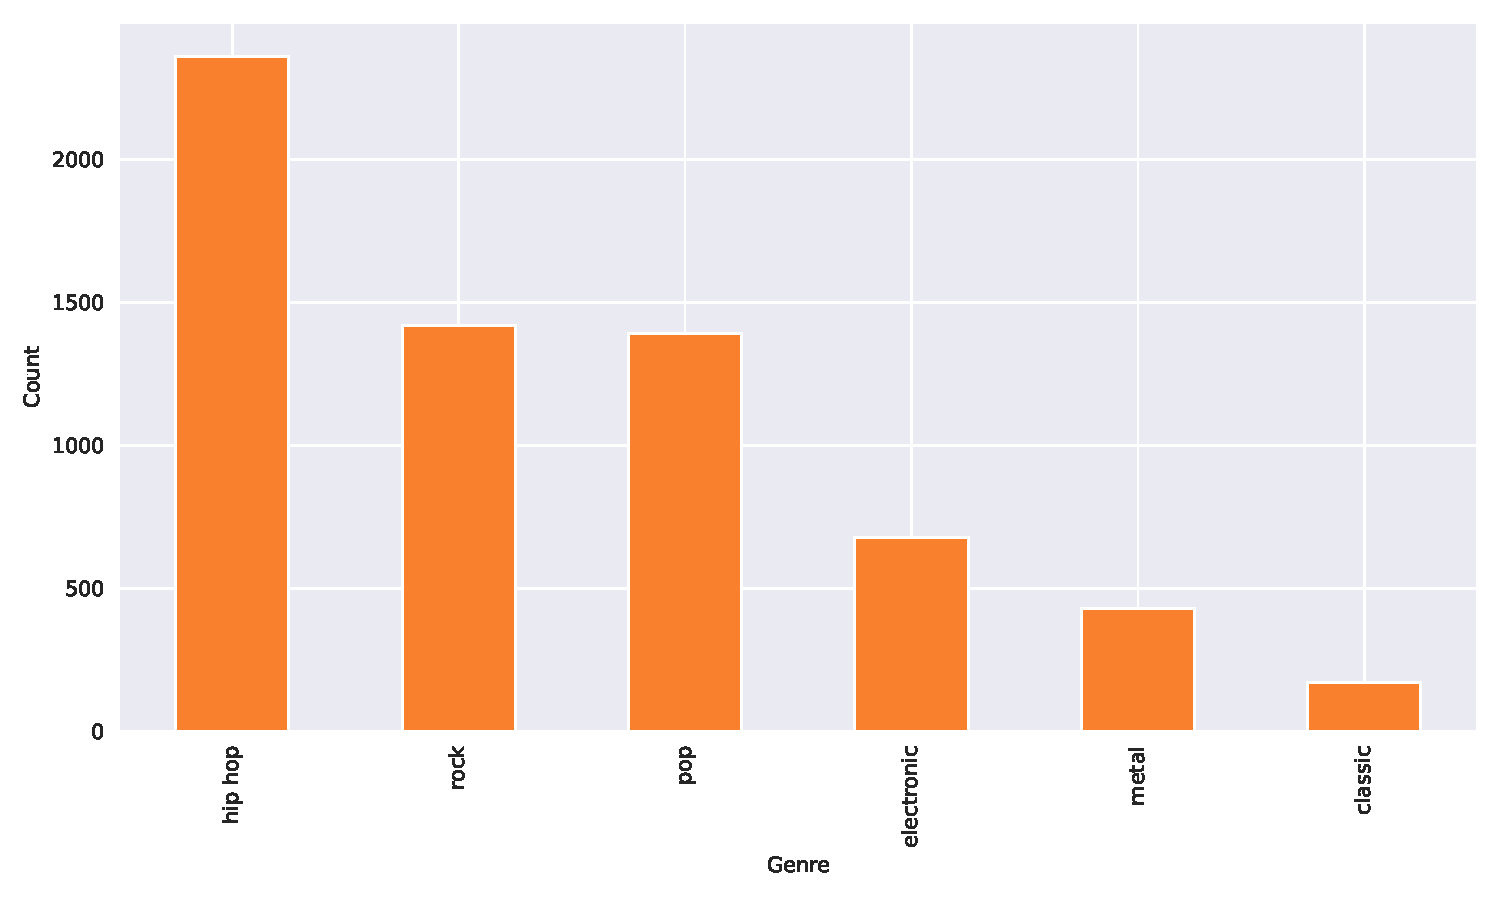
\includegraphics[scale=0.5]{figures/genre_hist_orange.pdf}
  \caption{Class imbalance of the resulting dataset.}
  \label{fig:class-imbalance}
\end{figure}
\FloatBarrier
Upon application of the preprocessing steps, the dataset is reduced to $6446$ entries.
\section{The dense Neural Network Model}
% a. Implementierung: Beschreibung der Implementierung des neuronalen Netzwerks.
% b. Ergebnisse: Wie hat das neuronale Netzwerk im Vergleich zu den anderen Methoden abgeschnitten?
% c. Diskussion: Warum hat das neuronale Netzwerk besser oder schlechter abgeschnitten?
\subsection{Architecture and Implementation}
The neural network used to solve this task conssits of...
\subsection{Performance and Results}

\section{Alternative Approaches to the Problem}
% a. Leistung von Knn: Wie hat das Knn-Modell abgeschnitten?
% b. Leistung von SVM: Wie hat das SVM-Modell abgeschnitten?
% c. Diskussion: Vergleich der beiden Modelle auf der Grundlage ihrer Ergebnisse.

\section{Discussion and Insights}
% a. Allgemeine Diskussion: Zusammenfassung der Erkenntnisse aus dem Projekt.
% b. Schlussfolgerungen: Was sind die endgültigen Schlussfolgerungen aus dem Projekt?
% c. Zukünftige Arbeiten: Gibt es Bereiche, in denen weitere Arbeit durchgeführt werden könnte?

\printbibliography

\end{document}
